Nessa seção vamos falar sobre o algoritmo guloso para o problema dos $k$-centros. Esse algoritmo foi desenvolvido pelo González~\cite{GONZALEZ1985293} e foi estudado na Seção 2.2 do livro WS2011.


A ideia desse algoritmo guloso se concentrará em, a cada iteração, escolher o vértice mais distante do conjunto de centros de clusters escolhidos até aquele momento para entrar no conjunto. Começaremos com um vértice arbitrário e iremos continuar inserindo novos centros de clusters até que tenhamos $k$ deles.

\begin{algorithm}
\caption{\sc Guloso-González$(G,c,k)$}
    \label{k-center:guloso}
    \begin{algorithmic}[1]
  \State Escolha arbitrariamente $u \in V(G)$.
        \State $S \gets \{u\}$.
        \While{$|S| < k$}
        \State $v \gets \arg\max_{j \in V(G)} c(j,S)$
        \State $S \gets S \cup \{v\}$
        \EndWhile
  \State \Return $S$.
\end{algorithmic}
\end{algorithm}

\begin{theorem}
    O algoritmo {\sc Guloso-González}$(G,c,k)$ é uma $2$-aproximação do problema dos $k$-centros métrico.
\end{theorem}
\begin{proof}
    É evidente que o algoritmo roda em tempo polinomial. 
  
    Seja $S^*$ uma resposta ótima de $I = (G,c,k)$ e $S$ o conjunto devolvido pelo algoritmo {\sc Guloso-González} para a instância $I$. Vamos mostrar que raio$(S) \leq 2\,\text{raio}(S^*) $. Seja $v \in S^*$ e ${u_1,u_2 \in V \setminus S}$ dois vértices tais que $ v = \arg\min_{i \in S} c_{iu_1} = \arg \min_{ i\in S} c_{iu_2}$, ou seja, dois vértices no mesmo cluster que $v$. Vale que
    \begin{align}
      c_{u_1u_2} \leq c_{u_1v} + c_{v u _2} = c(u_1,S) + c(u_2,S) \leq 2\, \text{raio}(S^*), \nonumber
    \end{align}
    em que a primeira desigualdade vale pela desigualdade triangular e a última desigualdade vale pela definição de raio$(S^*)$. Assim, a distância entre quaisquer dois vértices de um mesmo cluster é no máximo duas vezes o raio daquele cluster que por sua vez é no máximo raio$(S^*)$.
    Assim, se há exatamente um vértice de $S$ em cada cluster de $S^*$, então todos os vértices estão ligados com uma aresta de custo no máximo $2\,\opt(I)$ a um vértice de $S$. Então raio$(S) \leq 2\,\opt(I)$. Senão, seja $S_{i-1} \coloneqq \{ u_0,u_1,\ldots,u_{i-1}\}$ o conjunto $S$ ao final da iteração $i-1$ do laço {\bf Enquanto} da linha 3 e suponha que cada $u_j$ está em um cluster diferente de $S^*$ para $j = 1, \ldots, i-1$. Seja $u_i$ o vértice escolhido na iteração $i$ e suponha que ele está no mesmo cluster em $S^*$ que um vértice $u_j$ para algum $j<i$. Note que raio$(S_{i-1}) = c(u_i,S_{i-1}) \leq c_{u_iu_j}$, em que a primeira igualdade vale pela escolha feita na linha 4 e a segunda igualdade vale pela definição de $c(u_i,S_{i-1})$. Como $u_i$ e $u_j$ estão no mesmo cluster em $S^*$, vale que $c_{u_iu_j} \leq 2\,\text{raio}(S^*)$. Desse modo, concluímos que $\text{raio}(S) \leq \text{raio}(S_{i-1}) \leq 2\, \opt(I)$.
    
    
    %Então, $c(u_i,S_{i-1}) \leq c(u_iu_j) \leq 2\opt(I)$. Como $u_i$ maximiza $c(v,S_{i-1})$, então raio$(S) \leq 2\opt(I)$.
\end{proof}

Vamos mostrar que essa análise é justa, ou seja, existe uma instância $I = (G,c,k)$ em que o algoritmo devolve uma solução $S$ tal que raio$(S) = 2 \,\opt(I)$. 

Seja $G$ um grafo com pelo menos $k+2$ vértices em que as arestas têm custo 1 ou~2. O grafo induzido pelas arestas de custo 1 é uma estrela, como mostrado na figura abaixo.
\[
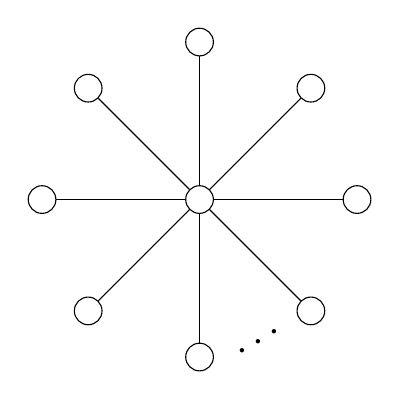
\begin{tikzpicture}
    % Number of outer vertices in the star
    \def\n{8}
    
    % Radius of the star
    \def\r{2cm}
    
    % Rotation angle
    \def\rotationangle{90}
    
    % Draw the central vertex
    \draw (0,0) node[circle, draw, minimum size=10pt, inner sep=1.5pt] (center) {};
    
    % Draw the outer vertices, rotated
    \begin{scope}[rotate=\rotationangle]
      \foreach \i in {1,...,\n} {
        \draw (\i*360/\n:\r) node[circle, draw, minimum size=10pt, inner sep=1.5pt] (\i) {};
      }
    \end{scope}
    
    % Connect the central vertex to every outer vertex
    \foreach \i in {1,...,\n} {
      \draw (center) -- (\i);
    }
    \draw (4) node[shift={(0.75,0.2)}] {\rotatebox{30}{\scalebox{1.5}{$\ldots$}}} (4);
  \end{tikzpicture}
  \]

  Claramente, o raio de uma resposta ótima dessa instância é 1 e inclui o vértice do centro da estrela como um dos centros de cluster.
  Note que se, no algoritmo guloso, o vértice escolhido arbitrariamente for algum dos vértices da ponta dessa estrela o vértice do centro nunca será escolhido, uma vez que ele nunca maximizará a função $c(j,S)$ na linha 4 do algoritmo. Assim, serão escolhidos apenas vértices da ponta da estrela e como temos pelo menos $k+1$ delas, sempre existirá um vértice ligado ao centro do seu cluster com uma aresta de custo 2.